\documentclass[twocolumn]{article}
\usepackage[english]{babel}
\usepackage[utf8]{inputenc}
\usepackage{amsmath,amssymb,physics,mathtools,blindtext,graphicx,float}
\usepackage[a4paper,total={7.5in,10in}]{geometry}
\usepackage[labelfont=bf]{caption}

\begin{document}
\begin{large}

\section*{TOV}
\subsection*{Introduction}
\begin{equation}
    \begin{split}
        &\frac{\text{d}P}{\text{d}r} = -\frac{G\left[P+\mathcal{E}(r)\right]\left[M(r)+4\pi r^3P/c^2\right]}{c^2r^2[1-2GM(r)/(c^2r)]} \\ 
        &\frac{\text{d}M}{\text{d}r} = 4\pi r^2\frac{\mathcal{E}(r)}{c^2}
    \end{split}
\end{equation}
An interpretation of these equations can be more readily seen by multiplying the first equation by $4\pi r^2\mathcal{E}\text{d}r/c^2 = \text{d}M$ and cancelling $\mathcal{E}$ on both sides:
\begin{equation}
    \begin{split}
        4\pi r^2\text{d}P &= -\frac{GM\text{d}M}{r^2}\left(1+\frac{P}{\mathcal{E}(r)}\right)\left(1+\frac{4\pi r^3P}{Mc^2}\right) \\ 
        &\hspace{2cm}\times\left(1-\frac{2GM}{c^2r^2}\right)^{-1}
    \end{split}
\end{equation}
The term on the left hand side is the force exerted on a infinitesimal shell at radius $r$. The first factor on the right hand side is the newtonian gravitational force from the interior acting on this shell.

\begin{equation}
    \label{24maj2054}
    \begin{split}
        &\mathcal{E}(n) = \frac{(mc^2)^4}{8\pi^2(\hbar c)^3}\bigg[x_F\sqrt{1+x_F^2}\left(1+2x_F^2\right) \\ 
        &\hspace{2.75cm}-\ln\left(x_F+\sqrt{1+x_F^2}\right)\bigg] \\ 
        &P(n) = \frac{(mc^2)^4}{8\pi^2(\hbar c)^3}\bigg[\frac{2}{3}x_F^3\sqrt{1+x_F^2}-x_F\sqrt{1+x_F^2} \\ 
        &\hspace{2.90cm}+\ln\left(x_F+\sqrt{1+x_F^2}\right)\bigg]
    \end{split}
\end{equation}
where $x_F(n)=\hbar c(3\pi n)^{1/3}/(mc^2)$.

\subsection*{Numerical set-up}
The TOV-equations can be made more suitible for numerical calculations by rescaling the variables. Making the substitutions $r = R_0x$, $P=P_0p$, $\mathcal{E} = \mathcal{E}_0\varepsilon$ and $M = M_0m$, the equation for the pressure can be written 
\begin{equation}
    \begin{split}
        &\left(\frac{P_0}{R_0}\right)\frac{\text{d}p}{\text{d}x} = -\left(\frac{GP_0M_0}{c^2R_0^2}\right) \\ 
        &\hspace{1cm}\times \frac{\left[p+(\mathcal{E}_0/P_0)\varepsilon\right]\left[m+4\pi R_0^3x^3P_0p/(c^2M_0)\right]}{x^2\left[1-2GM_0m/(c^2R_0x)\right]}.
    \end{split}
\end{equation}
Cancelling $P_0/R_0$ on both sides yields
\begin{equation}
    \begin{split}
        &\frac{\text{d}p}{\text{d}x} = -\left(\frac{G_0M_0}{c^2R_0}\right) \\ 
        &\hspace{1cm}\times \frac{\left[p+(\mathcal{E}_0/P_0)\varepsilon\right]\left[m+4\pi R_0^3x^3P_0p/(M_0c^2)\right]}{x^2\left[1-2GM_0m/(c^2R_0x)\right]}
    \end{split}
\end{equation}
Similarily, the equation for the mass becomes
\begin{equation}
    \frac{\text{d}m}{\text{d}x} = \left(\frac{4\pi R_0^3\mathcal{E}_0}{M_0c^2}\right)x^2\varepsilon
\end{equation}
The equations for $p$ and $m$ simplify substantially if the numerical constants are chosen such that
\begin{equation}
    \label{26maj1005}
    1 = \frac{\mathcal{E}_0}{P_0} = \frac{GM_0}{c^2R_0} = \frac{4\pi R_0^3P_0}{M_0c^2}.
\end{equation}
Then the TOV-equations become
\begin{equation}
    \label{24maj1640}
    \begin{split}
        &\frac{\text{d}p}{\text{d}x} = -\frac{(\varepsilon+p)(m+x^3p)}{x(x-2m)} \\  %= f(p,\epsilon,m;x) \\ 
        &\frac{\text{d}m}{\text{d}x} = x^2\varepsilon. %= g(\epsilon;x)
    \end{split}
\end{equation}
A natural choice for $\mathcal{E}_0$ and $P_0$ is the term in front of the brackets in \eqref{24maj2054}:
\begin{equation}
    \mathcal{E}_0 = P_0 = \frac{(mc^2)^4}{8\pi^2(\hbar c)^3} \approx 1.285 \text{ GeV/fm}^3.
\end{equation}
Equation \eqref{26maj1005} then fixes $M_0$ and $R_0$:
\begin{equation}
    \begin{split}
    &M_0 = \sqrt{\frac{c^8}{4\pi\mathcal{E}_0G^3}} \approx 4.63 \text{ M}_\odot \\ 
    &R_0 = \frac{GM_0}{c^2} \approx 6.84 \text{ km}
    \end{split}
\end{equation}
where M$_\odot$ is the mass of the sun.


To solve these equations, initial conditions for both $p$ and $m$ are needed. From a physical consideration it is obvious to set $m(0)=0$. The initial value for the pressure can be either $p(0) = p_0$ or $p(x_0) = 0$ where $p_0$ is the pressure at the center of the star and $x_0$ is its radius. When $\varepsilon$ depends on the pressure $p$, it becomes easier to make use of the former condition since $m$ is integrated from the center. The equation for $p$ is however singular for $x=0$, so the equations have to be integrated from some value $\Delta x$ close to zero. Since the first two derivatives of $m$ are zero at $x=0$, the error of setting $m(\Delta x) = 0$ is of the order $(\Delta x)^3$.

Another thing which is needed is the equation of state $\epsilon(p)$ which, for the case of an ideal Fermi gas at zero temperature, can not be found directly but in terms of the number density $n$:
\begin{equation}
    \label{24maj1641}
    \begin{split}
        &\varepsilon(n) = x_F\sqrt{1+x_F^2}\left(1+2x_F^2\right)-\ln\left(x_F+\sqrt{1+x_F^2}\right) \\ 
        &p(n) = \frac{2}{3}x_F^3\sqrt{1+x_F^2}-x_F\sqrt{1+x_F^2} \\ 
        &\hspace{3.75cm}+\ln\left(x_F+\sqrt{1+x_F^2}\right)
    \end{split}
\end{equation}
with $x_F(n)=\hbar c(3\pi n)^{1/3}/(mc^2)$. Hence, for a given $p=p_0$ we need a root finding algorithm to find $n=n_0$ such that $p(n_0) = p_0$. Once $n_0$ has been found, we can plug that into $\varepsilon$ to find $\varepsilon(n_0)=\varepsilon(p_0)$. 

Having set up the equations which are to be integrated \eqref{24maj1640} and the equation of state \eqref{24maj1641}, the following steps were taken to solve the TOV-equations: 
\begin{itemize}
    \item[1.] Set the initial conditions by specifying $p(\Delta x) = p_c = p_{j=0}$ and set $m(\Delta x) = 0 = m_{j=0}$.
    \item[2.] Find the energy density by using the bisection method on $p(n) = p_j$ and plugging $n$ into the equation for the energy density to get $\epsilon(n)=\varepsilon_j$. 
    \item[3.] Use Heun's integration method on \eqref{24maj1640} to obtain $p_{j+1}$ and $m_{j+1}$. 
    \item[4.] Repeat from 2. until the pressure is zero, $p_{j+1}=0$.
\end{itemize}
The step size used was $h=10^{-4}$ and the tolerance for the bisection method was $\Delta = 10^{-8}$. 

\subsection*{Results}
\begin{center}
    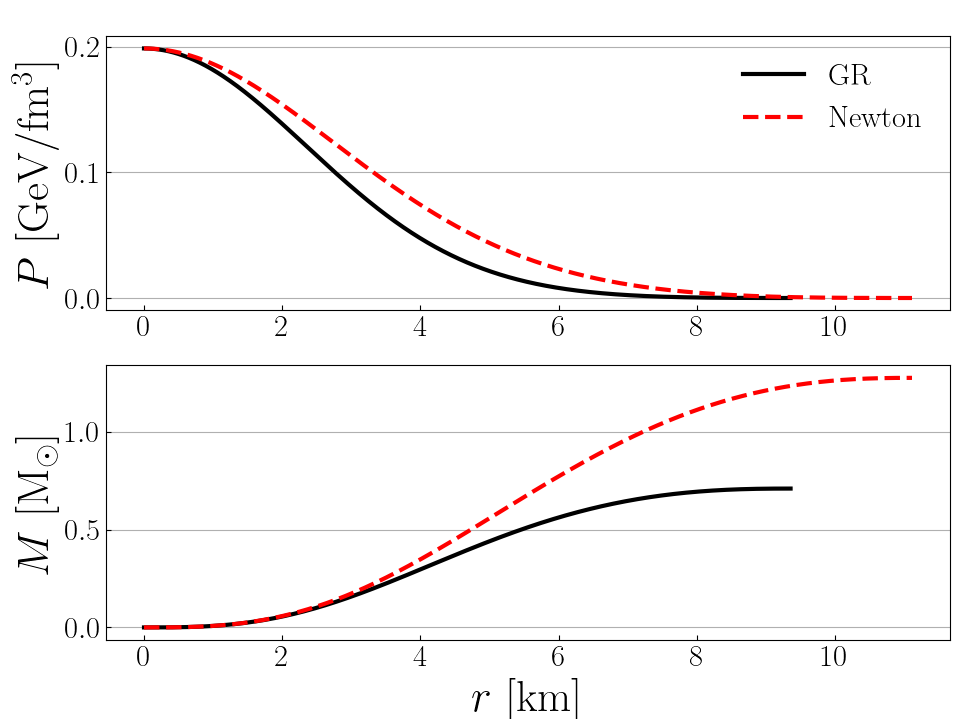
\includegraphics[scale=0.35]{Newt.png}
\end{center}
\begin{center}
    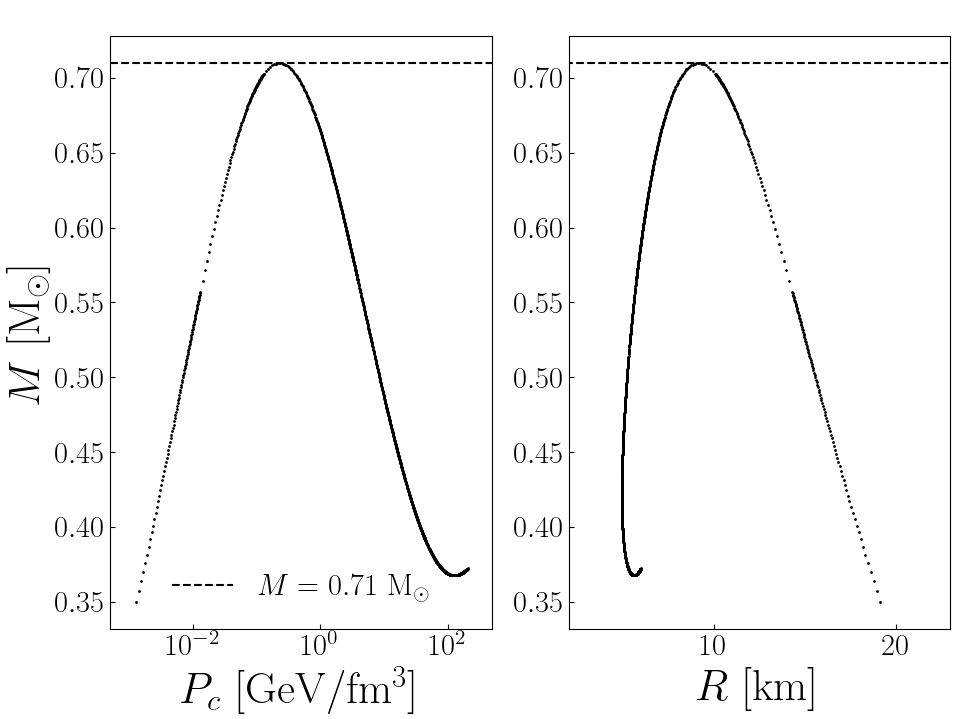
\includegraphics[scale=0.35]{TOV_limit.png}
\end{center}



\subsection*{Notes}
\begin{itemize}
    \item Compare with Newton
    \item Also do white dwarfs
\end{itemize}




\end{large}
\end{document}
